\problemname{Quicksand}
\noindent

\illustration{0.24}{sand.jpg}{\href{https://commons.wikimedia.org/wiki/File:Morocco_Africa_Flickr_Rosino_December_2005_84527213.jpg}{Sand}, CC BY-SA 2.0}

Sandra has moved to Sandsvall to study. After spending a few days in the new city, Sandra has noticed that there is quicksand in several locations. If you go to any of these locations, you get stuck in the sand and cannot escape. Sandra wants to know exactly where the quicksand is located so she can avoid these places. Fortunately, unlike Gothenburg, Sandsvall has a well-functioning travel planning app. Using the travel planner, Sandra has found out how long it takes to travel from her residence to each of the other locations in the city.

Sandsvall can be represented by a grid with $N$ rows and $M$ columns. Sandra's residence is in one of the cells of this grid. It takes one minute to travel between two adjacent cells (two cells are adjacent if they share at least one of the 4 sides). In some cells, there is quicksand, and it is impossible to travel from those cells at all.

Let $(r, c)$ be the cell at row $r$ and column $c$. You are given the number $d_{r,c}$ for each cell in the grid, which represents the minimum possible number of minutes it takes to travel from Sandra's residence to that cell. Your task is to handle $Q$ queries of the following types:

\begin{itemize}
    \item \verb|? r c|: Determine if there is quicksand in cell $(r, c)$. You should answer \verb|ja| (yes), \verb|nej| (no), \verb|kanske| (maybe), or \verb|fel| (error).
    \item \verb|! r c d|: Change the value of $d_{r, c}$ to $d$.
\end{itemize}

\section*{Input}

The first line contains three integers $N$, $M$, and $Q$ ($1 \leq N,M,Q \leq 3 \cdot 10^5$, $N\cdot M \leq 3 \cdot 10^5$).

The following $N$ lines contain $M$ integers each. The $i$-th of these lines contains the integers $d_{i,1}, d_{i,2}, d_{i,3}, \dots d_{i,M}$ ($-1 \leq d_{i,j} \leq 3 \cdot 10^5$).

There will be exactly one cell that satisfies $d_{r, c} = 0$, which is Sandra's residence. If $d_{r, c} = -1$, it means that it is impossible to reach cell $(r, c)$ at all.

The following $Q$ lines contain the queries to be processed, in the format described above. 
The numbers $r, c$ that appear in the queries satisfy $1 \leq r \leq N$ and $1 \leq c \leq M$. 
The numbers $d$ that appear satisfy $-1 \leq d \leq 3 \cdot 10^5$, $d \neq 0$. 
Sandra's residence will always have a distance of zero, and no other cell's distance will be changed to zero.

\section*{Output}

Write the answer to each query of the form \verb|? r c|.
\begin{itemize}
  \item If there is no way to distribute the quicksand that is consistent with the given numbers $d$, you should output \verb|fel|.
  \item Otherwise, if there must be quicksand in cell $(r, c)$, output \verb|ja|.
  \item If there is guaranteed to be no quicksand in cell $(r, c)$, output \verb|nej|.
  \item If it is both possible and not possible for there to be quicksand in cell $(r, c)$, output \verb|kanske|.
\end{itemize}

\section*{Scoring}
Your solution will be tested on a set of test groups, each worth a number of points. Each test group contains
a set of test cases. To get the points for a test group you need to solve all test cases in the test group.

\noindent
\begin{tabular}{| l | l | p{12cm} |}
  \hline
  \textbf{Group} & \textbf{Points} & \textbf{Constraints} \\ \hline
  $1$    & $17$        & $N = 1$ \\ \hline
  $2$    & $28$        & $N,M,Q \leq 100$ \\ \hline
  $3$    & $20$        & The answer is never \verb|fel|. \\ \hline
  $4$    & $35$        & No additional constraints. \\ \hline
\end{tabular}

\section*{Explanation of Sample}

\begin{figure}[h!]
  \centering
  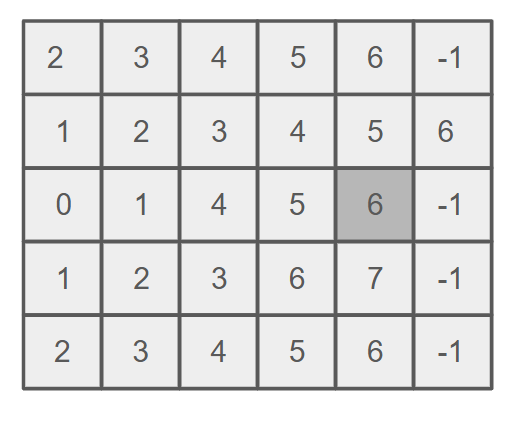
\includegraphics[width=0.35\textwidth]{kvicksand2.PNG}
\end{figure}

This is what the grid looks like in the sample case. In the first query, we need to determine if $(3, 5)$ (highlighted in gray) has quicksand, and it must have it. In the third query, we need to determine if $(1, 6)$ has quicksand, and it is impossible to determine because it is unreachable. After the update that changes the value of $(5, 4)$ to $7$, the distances no longer correspond to any valid distribution of quicksand.